
\documentclass[12pt]{extarticle}
\usepackage{comands} 
\usepackage{chronology}

\title{\LARGE 
Lenguajes de Programación 2023-1\\ 
Nota de clase 6: Estrategias de evaluación \\
\color{SeaGreen} Funcional ($\lambda$)}
\author{Javier Enríquez Mendoza }
\date{\today}

\begin{document}

\maketitle 

En la nota de clase anterior vimos que la regla de $\beta$-reducción, define una semántica operacional para el Cálculo Lambda, sin embargo esta regla de reducción es no determinista. En la teoría el no determinismo de las funciones de reducción no representa un problema siempre que éstas sean confluentes, sin embargo, en la implementación de un interprete para el lenguaje este no determinismo representa un problema mucho mas grave pues en la mayoría de los lenguajes no hay forma de representar esta característica y mas aún el interprete puede reaccionar de forma inesperada. Es por esto que el no determinismo nos impide utilizar al Cálculo Lambda por si sólo como un lenguaje de programación. 

Eliminar el no determinismo de las funciones de reducción es en la mayoría de los casos una tarea compleja y no siempre posible, por lo que para solucionar este problema se opta por la implementación de interpretes simbólicos para los lenguajes en donde implícitamente se elije un camino a seguir en el proceso de evaluación siempre utilizando el mismo criterio para la elección del estado siguiente cuando haya mas de uno posible. Estos criterios son lo que se conoce como estrategias de evaluación.

Si bien estas estrategias son definidas en el Cálculo Lambda pueden extenderse a cualquier lenguaje de programación, y son estrategias que se utilizan en la actualidad para la definición de la semántica operacional de los lenguajes para lograr el determinismo de ésta.

\section{Reducción no determinista}

La semántica operacional propuesta para el Cálculo Lambda es no determinista, pero solo lo es en el proceso que se sigue para evaluar una expresión, no en el resultado final de ésta, gracias a la propiedad de confluencia que garantiza la unicidad de las formas normales de los lambda términos. Que gráficamente se ve como a sigue:

\begin{center}
\begin{tikzpicture}[node distance={25mm}, thick, main/.style = {}] 
\node[main] (1) {$t$}; 
\node[main] (2) [below left of=1]{$t_1$}; 
\node[main] (3) [below right of=1] {$t_2$}; 
\node[main] (4) [below right of=2] {$t_f$}; 
\draw[->] (1) -- (2); 
\draw[->] (1) -- (3);
\draw[->] (2) -- (4);
\draw[->] (3) -- (4);
\end{tikzpicture} 
\end{center}
\noindent
Que se lee como: Siempre que $t\to^\star_\beta t_1$ y $t\to^\star_\beta t_2$ existe un lambda término $t_f$ tal que $t_1\to^\star_\beta t_f$ y $t_2\to^\star_\beta t_f$ y $t_f$ está en forma normal.

A pesar de que nos resulta mas intuitivo pensar en una evaluación determinista, existen algunas razones para considerar un proceso de evaluación no determinista, por ejemplo, el diseñar una semántica operacional no determinista da una mayor flexibilidad al compilador de aplicar optimizaciones sobre el programa, como puede ser la eliminación de subexpresiones idénticas, de tal forma que se evalúe una única vez cada subexpresión a pesar de estar presente en mas de una ocasión en el programa.

Otra ventaja de las semánticas no deterministas es el paralelismo, si podemos evaluar las subexpresiones del programa en cualquier orden, entonces es posible evaluar mas de una expresión de forma paralela sin afectar el resultado final, esto mejora la eficiencia con la que se ejecutan los programas de nuestro lenguaje.

\section{Estrategias de reducción}

En esta sección estudiaremos la definición de distintos interpretes deterministas para el Cálculo Lambda, en donde para cada uno se elije una estrategia de evaluación para eliminar el no determinismo de la $\beta$-reducción.

\begin{definition}[Estrategia de evaluación] Una estrategia de evaluación es una función parcial $F$ de términos a términos con la propiedad de que si $F(t)=t'$ entonces $t\to_\beta t'$. Y se la llama estrategia pues $F$ podría utilizarse para elegir una de las posibles reducciones para $t$.
\end{definition}

\begin{definition}[Reducción determinista]
Para cada estrategia de evaluación $F$ se puede definir recursivamente una función de reducción determinista $\to_F$ de la siguiente forma:
\[
	t \to_F \begin{cases}
	  t  & \text{si }F(t)\text{ no está definida} \\
	  t_f & \text{si }F(t)=t'\text{ y }t'\to_F t_f
	\end{cases}
\]

Ahora presentamos $\to_F$ como una definición inductiva con reglas de inferencia:
\[
	\begin{array}{ccc}
	\inference{F(t)={\tt undef}}{t\to_F t}&
	\quad\quad&
	\inference{F(t)=t'&t'\to_F t_f}{t\to_F t_f}
	\end{array}
\]
\noindent
De esta forma $\to_F$ es una función de evaluación determinista que aplica reducciones paso a paso siguiendo la estrategia $F$ hasta que ya no es posible.
\end{definition}

Para el diseño de la semántica operacional de un lenguaje de programación en general nos van a interesar estrategias de evaluación que nos ayuden a reducir las expresiones para llegar a su forma normal.

Una característica importante de las estrategias de evaluación es que en la mayoría de los casos no son únicas, es decir, para un mismo lenguaje se pueden definir mas de una estrategia de evaluación. 

\begin{example}[Estrategias de evaluación en Cálculo Lambda]
Por ejemplo, consideremos la siguiente expresión del Cálculo Lambda: $(\lambda x.{\sf N}){\sf M}$ en donde ${\sf N}\to_\beta{\sf N'}$ y ${\sf M}\to_\beta{\sf M'}$, entonces tenemos tres alternativas de elección para el siguiente paso en la evaluación de la expresión, las cuales se muestran en el diagrama siguiente:

\begin{center}
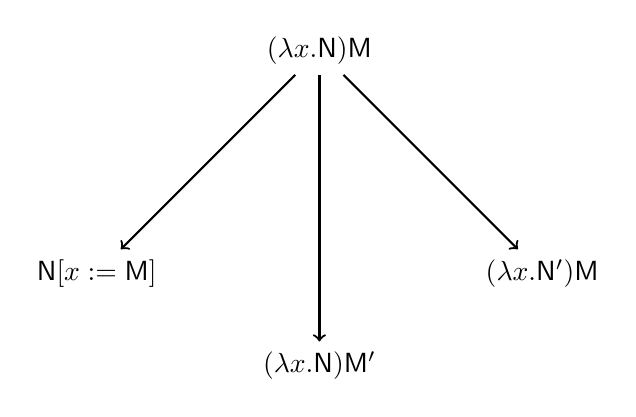
\begin{tikzpicture}[node distance={40mm}, thick, main/.style = {}] 
\node[main] (1) {$(\lambda x.{\sf N}){\sf M}$}; 
\node[main] (2) [below left of=1]{${\sf N}[x := {\sf M}]$}; 
\node[main] (3) [below right of=1] {$(\lambda x.{\sf N'}){\sf M}$}; 
\node[main] (4) [below of=1] {$(\lambda x.{\sf N}){\sf M'}$}; 
\draw[->] (1) -- (2); 
\draw[->] (1) -- (3);
\draw[->] (1) -- (4);
\end{tikzpicture} 
\end{center}

Cada una de estas opciones define una estrategia de evaluación distinta:
\begin{itemize}
\item La primera se le llama {\it evaluación perezosa} en donde el argumento de la función se sustituye sin ser evaluado previamente.
\item La segunda recibe el nombre de {\it evaluación ansiosa} en donde el argumento de la función es evaluado antes de pasarlo.
\item Y la tercera puede verse como una optimización sobre la función $(\lambda x.{\sf N})$ para intentar reducirla antes de evaluar la aplicación.
\end{itemize}
\end{example}

La evaluación ansiosa, en la que se reduce el parámetro de la función antes de hacer la $\beta$-reducción en algunos casos reduce los pasos de evaluación de una expresión. La razón es porque el cuerpo ${\sf N}$ de la función puede tener varias ocurrencias de la variable $x$ por lo que sustituirla directamente por la forma normal de ${\sf M}$ puede evitar múltiples reducciones del término ${\sf M}$.

Por el otro lado si $x$ no aparece en ${\sf N}$ no tiene sentido reducir ${\sf M}$, un caso especialmente importante de esto es cuando ${\sf M}$ no tiene forma normal, por ejemplo si ${\sf M} = \Omega$, con una estrategia ansiosa la evaluación diverge mientras que con la estrategia perezosa se llega a la forma normal de la expresión. 
\begin{description}
	\item[Evaluación Ansiosa]
	$$(\lambda x.{\sf N})\Omega\to_\beta(\lambda x.{\sf N})\Omega\to_\beta(\lambda x.{\sf N})\Omega\to_\beta(\lambda x.{\sf N})\Omega\to_\beta\cdots$$
	\item[Evaluación Perezosa]
	$$(\lambda x.{\sf N})\Omega\to_\beta{\sf N}$$
\end{description}

Con estos ejemplos podemos notar que no hay una estrategia correcta, sino que cada una tiene sus ventajas y desventajas, las cuales serán estudiadas con mayor profundidad en las siguientes secciones de la nota.

\subsection{Evaluación perezosa}

La \textbf{evaluación perezosa} (del inglés \textit{lazy evaluation}) o llamada por necesidad es una estrategia de evaluación que retrasa el cálculo de una expresión hasta que su valor sea necesario, y que también evita repetir la evaluación en caso de ser necesaria en posteriores ocasiones. Esta compartición del cálculo puede reducir el tiempo de ejecución de ciertas funciones de forma exponencial, comparado con otras estrategias de evaluación.

Los beneficios de la evaluación perezosa son:

\begin{itemize}
    \item El incremento en el rendimiento al evitar cálculos innecesarios, y en tratar condiciones de error al evaluar expresiones compuestas.
    \item La capacidad de construir estructuras de datos potencialmente infinitas.
    \item La capacidad de definir estructuras de control como abstracciones, en lugar de operaciones primitivas.
\end{itemize}

A continuación se define una semántica operacional para el Cálculo Lambda usando esta estrategia de evaluación.

\begin{definition}[Función de evaluación determinista perezosa] Se extiende la $\beta$-reducción con las siguientes reglas que modelan la estrategia de evaluación perezosa:
\[
	\begin{array}{ccc}
	\inference{t_1\to_{lazy}t_1'}{t_1\;t_2\to_{lazy}t_1'\;t_2}&
	\quad\quad&
	\inference{}{(\lambda x.t_1)t_2\to_{lazy}t_1[x:=t_2]}
	\end{array}
\]
\end{definition}

\begin{example}[Proceso de evaluación] A continuación se presenta la evaluación de un lambda término usando la estrategia de evaluación perezosa.

\[
\begin{array}{rl}
&(\lambda x.(\lambda y. y) x)(\lambda z.(\lambda w. ww) z)\\
\to_{lazy}&(\lambda x.x)(\lambda z.(\lambda w. ww) z)\\
\to_{lazy}&(\lambda z.(\lambda w. ww) z)\\
\to_{lazy}&(\lambda z.zz)\\
\end{array}
\]
\end{example}
\subsection{Evaluación ansiosa}

La \textbf{evaluación ansiosa} (del inglés \textit{eager evaluation}), también conocida como evaluación estricta o evaluación codiciosa, es la estrategia de evaluación utilizada por la mayoría de los lenguajes de programación tradicionales. En la evaluación ansiosa, una expresión se evalúa tan pronto como se vincula a una variable. 

Los efectos de la evaluación ansiosa incluyen:

\begin{itemize}
    \item Código fácilmente comprensible en términos de orden de ejecución que no cambia potencialmente su comportamiento basado en un cambio de contexto de ejecución.
    \item Un proceso de depuración más fácil en comparación con otras estrategias de evaluación debido a lo anterior.
    \item Sin embargo, la responsabilidad del rendimiento del código se desplaza hacia el programador, por lo que se requiere un cuidadoso proceso de optimización del código.
\end{itemize}

Ahora definimos la semántica operacional del Cálculo Lambda correspondiente con esta estrategia de evaluación.
\begin{definition}[Función de evaluación determinista ansiosa] Se extiende la $\beta$-reducción con las siguientes reglas que modelan la estrategia de evaluación ansiosa:
\[
	\begin{array}{ccc}
	\inference{t_1\to_{eager}t_1'}{t_1\;t_2\to_{eager}t_1'\;t_2}&
	\quad\quad&
	\inference{t_2\to_{eager}t_2'}{(\lambda x.t_1)t_2\to_{eager}(\lambda x.t_1)t_2'}
	\end{array}
\]
\end{definition}
\begin{example}[Proceso de evaluación] A continuación se presenta la evaluación de un lambda término usando la estrategia de evaluación ansiosa.

\[
\begin{array}{rl}
&(\lambda x.(\lambda y. y) x)(\lambda z.(\lambda w. ww) z)\\
\to_{eager}&(\lambda x.x)(\lambda z.(\lambda w. ww) z)\\
\to_{eager}&(\lambda x.x)(\lambda z.zz)\\
\to_{eager}&(\lambda z.zz)\\
\end{array}
\]
\end{example}
\subsection{Evaluación en paralelo}

La {\bf Evaluación en paralelo} es una estrategia de evaluación en donde todas las subexpresiones del término son evaluadas simultáneamente.

Este tipo de evaluación no siempre es posible de definir, pues en lenguajes con efectos secundarios puede afectar el resultado del cómputo que se está evaluando. Esto hace que no sea muy común en lenguajes de programación reales. Es mas que nada utilizada como optimización del proceso de evaluación sobre subconjuntos de los lenguajes de programación con evaluación ansiosa.

La principal ventaja de esta estrategia es que mejora considerablemente el tiempo de evaluación de los programas. También cuenta con las mismas ventajas que la evaluación ansiosa, es por esto que en la literatura se puede encontrar como una variante de la evaluación ansiosa en lugar de verla como una estrategia diferente.

\begin{definition}[Función de evaluación determinista paralela] Se extiende la $\beta$-reducción con las siguientes reglas que modelan la estrategia de evaluación paralela:

\[
	\begin{array}{c}
	\inference{t_1\to_{par}t_1'&t_2\to_{par}t_2'}{t_1\;t_2\to_{par}t_1'\;t_2'}
	\end{array}
\]
\end{definition}
\begin{example}[Proceso de evaluación] A continuación se presenta la evaluación de un lambda término usando la estrategia de evaluación en paralelo.

\[
\begin{array}{rl}
&(\lambda x.(\lambda y. y) x)(\lambda z.(\lambda w. ww) z)\\
\to_{par}&(\lambda x.x)(\lambda z.zz)\\
\to_{par}&(\lambda z.zz)\\
\end{array}
\]
\end{example}

\section{Propiedades de las estrategias de evaluación}
Las estrategias de evaluación son un mecanismo que nos permiten implementar interpretes simbólicos de forma determinista, sin embargo es importante que éstas no cambien la semántica de los lenguajes, por lo que la evaluación usando estrategias y sin ellas debe obtener el mismo resultado, lo que se expresa con la siguiente propiedad:

\begin{proposition}[Correctud de las estrategias de evaluación] Sean $F$ una estrategia de evaluación y $t$ y $t_f$ lambda términos tal que $t\to^\star_Ft_f$  y $t_f\not\to_F$ entonces $t\to^\star_{\beta}t_f$ y $t_f\not\to_\beta$. Es decir, la forma normal de una expresión calculada con la estrategia $F$ es igual a la obtenida a partir de la regla de $\beta$-reducción.
\end{proposition}
\begin{proof}
Inducción sobre las reglas de reducción de $\to_F$.
\end{proof}
Con la propiedad anterior podemos ayudarnos de las estrategias de evaluación en la definición de la semántica operacional de un lenguaje de programación, ahora solo falta demostrar que dichas estrategias cumplen su cometido de garantizar el determinismo de la evaluación de una expresión.
\begin{proposition}[Determinismo de las estrategias de evaluación] Sea $F$ una estrategia de evaluación, entonces si $t\to_F t_1$ y $t\to_F t_2$ se cumple que $t_1 = t_2$, es decir, la función de reducción $\to_F$ es determinista.
\end{proposition}
\begin{proof}
Inducción sobre las reglas de reducción de $\to_F$.
\end{proof}

\begin{thebibliography}{9}


\bibitem{mitchell}
Mitchell J., Foundations for Programming Languages. MIT Press 1996.

% \bibitem{notasGabrielle}
% Keller G., O'Connor-Davis L., Class Notes from the course Concepts of programming language design, Department of Information and Computing Sciences, Utrecht University, The Netherlands, Fall 2020.

\bibitem{notasFavio}
Miranda Perea F., González Huesca L., Nota de Clase del curso de Lenguajes de Programación, Facultad de Ciencias UNAM, Semestre 2021-1.

\bibitem{notasKarla}
Ramírez Pulido K., Soto Romero M., Nota de Clase del curso de Lenguajes de Programación, Facultad de Ciencias UNAM, Semestre 2021-2

% \bibitem{harper}
% Harper R., Practical Foundations for Programming Languages. Working draft, 2010.


\bibitem{shriram}
Krishnamurthi S., Programming Languages Application and Interpretation; Version 26.04.2007.


\end{thebibliography}




\end{document}